\documentclass{article}
\usepackage{graphicx}
\usepackage{amsmath}
\usepackage{amsfonts}
\usepackage{graphicx}
\usepackage{hyperref}

\begin{document}

\title{Convolutional Neural Neural Network For Maze Solving}
\author{Axel Ind (\textit{4563539}), Fernando Cristiani \textit{(4527671)}}

\maketitle

\begin{abstract}
This document details work to create and evaluate a convolutional neural network that solves mazes with a partially observable environment. Training is conducted through problem simulation with the $A^*$ algorithm. The network architecture consisted of 2 convolutional layers, each followed by a pooling layer and a single fully connected softmax output layer. Training accuracy of $99.2\%$ is achieved for history $\geq 4$. Testing accuracy of $100\%$ is achieved for history $=2$.
\end{abstract}

\section{Dataset}
\subsection{Data Format}
Each input consists of 3-dimensional numeric input of depth $d$. The $25\times 25\times d$ matrix provides a instantaneous grayscale representation of the current state of the agent in the maze, and the same information for each of its last $d-1$ states. Individual values in the matrix range from $0$ to $255$ and are used to represent cell occupation.
\subsection{Data Generation}
Data is generated to mimic the performance of the $A^*$ algorithm. The \textit{get\_data.py} program generates a large dataset of time-delimited states as traversed by the $A^*$ agent. Further, this dataset provides only a local view of the map from the agent's perspective up to a parameter-defined depth.

\section{Network Architecture}
\subsection{Inputs}
\textbf{Stochastic Gradient Descent}: $25 \times 25 \times d \times n$ (where $d$ is the history length, $n$ is the batch size).

\subsection{Outputs}
$Y=(y_0, y_1, y_2, y_{3}, y_{4})$

\noindent
Each class corresponds to a classification of: $(0,4) \in \mathbb{Z} $.

\noindent
More precisely the actions are mapped as follows:

\noindent
\begin{tabular}{ |c|c|c| } 
 \hline
 \textbf{Action} & \textbf{Agent Motion} \\ 
 0 & Do nothing \\ 
 1 & Up \\ 
 2 & Down\\
 3 & Left \\ 
 4 & Right\\
 \hline
\end{tabular}

\section{Training}

\subsection{Propagation}
All training results are achieved using backpropagation to update weights.

\subsection{Testing Hyperparameters}
\begin{itemize}
\item \textbf{Network architecture}: $\textrm{Input}-\{\textrm{Conv-Relu-Pool}\}^2-\textrm{FullyConnectedLayer-Softmax}$
\item \textbf{NumFilters}: $32^{|1|},64^{|2|}$
\item \textbf{KernelSize}: $5\times 5$
\item \textbf{BatchSize}: $100$
\end{itemize}

\subsection*{Testing Architecture}




\begin{tabular}{ |c|c|c| } 
 \hline
 CPU & i7-6700HQ \\ 
 GPU & GTX970 (6GB) \\ 
 RAM & 16GB \\ 
 Hard Disk & SSD\\
 \hline
\end{tabular}





\section{Results}
\subsection{Local View Performance}
\subsubsection*{Training Accuracy}
\begin{figure}[ht]
\centering
  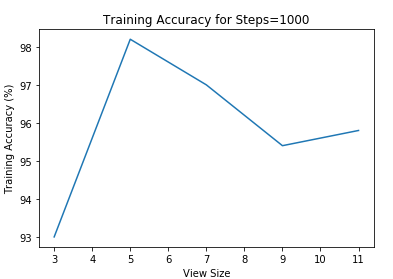
\includegraphics[width=0.6\linewidth]{trainingAccuracy_view}
  \caption{Graph showing the effect of varied view size on the training accuracy of the convolutional neural network.}
  \label{fig:trainingAccuracy_view}
\end{figure}
Figure~\ref{fig:trainingAccuracy_view} illustrates that the view size does not appear to increase training accuracy for a step count of $1000$. This may be a result of too few training iterations to properly train the increased number of parameters for the filters.

\subsubsection*{Testing Accuracy}
\begin{figure}[ht]
\centering
  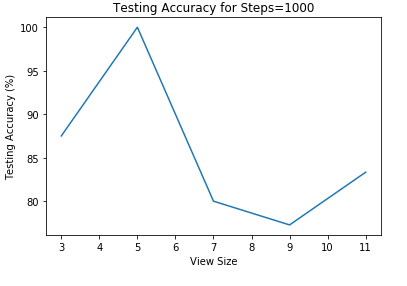
\includegraphics[width=0.6\linewidth]{testingAccuracy_view}
  \caption{Graph showing the effect of varied view size on the testing accuracy of the convolutional neural network.}
  \label{fig:testingAccuracy_view}
\end{figure}

Figure~\ref{fig:testingAccuracy_view} illustrates that the view size does not appear to increase testing accuracy for a step count of $1000$. This may be a result of too few training iterations to properly train the increased number of parameters for the filters.

In the case of testing, the optimal view size (i.e. the one that maximizes testing accuracy) appears to be $5\times5$. For a step count of $1000$, and history length of $4$ it returned an accuracy of $100.00\%$.

\subsection{Effect Of History Parameter}

\begin{figure}[ht]
\centering
  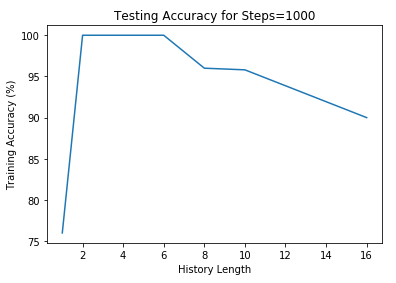
\includegraphics[width=0.6\linewidth]{testingAccuracy}
  \caption{Testing Accuracy for the CNN as measured by the probability of the agent reaching its goal in finite number of actions.}
  \label{fig:testingAccuracy}
\end{figure}

\begin{figure}[ht]
\centering
  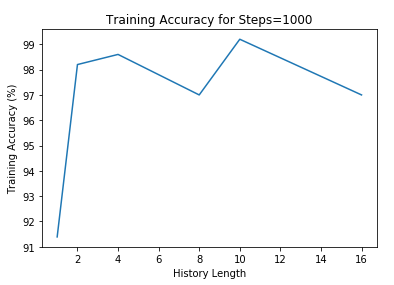
\includegraphics[width=0.6\linewidth]{trainingAccuracy}
  \caption{Training Accuracy for the CNN as compared to validation set. This figure only illustrates the frequency of the agent taking exactly the same action as the $A^{*}$ search.}
  \label{fig:trainingAccuracy}
\end{figure}

Figure~\ref{fig:trainingAccuracy}, taken in isolation, would appear to show that the predictive accuracy of the agent roughly converged for any history length $>2$. With a maximum predictive accuracy of $99.2\%$, it appears to very accurately match $A^*$ performance in training.

However, the true testing criteria is not finding an optimal action in any given state; it is finding the target within a finite number of actions. The relationship between history length and probability of reaching the target is illustrated in Figure~\ref{fig:testingAccuracy}.

In practice, it is observed that the agent successfully finds its goal $100\%$ of the time for history length of $2$ and $4$. It is the belief of the authors that the dramatic reduction in the test accuracy observed was the result of 2 separate factors.

First, the increased number of parameters required by the network for greater input depth may have required more training time than was allocated (steps$=1000$).

Second, and more significantly, the agent appears to interpret higher uncertainty in its current state when the history length is increased. One can only conjecture at how the nature of the non-convex loss function is affected by this dimensionality manipulation.

\subsection{Unknown Map Exploration} \label{ssec:unk}
As expected, unknown map exploration resulted in an extremely low testing accuracy ($\approx 0.2\%$ for $16$ random maps with reachable targets). 

\subsection{Unknown Target} \label{ssec:unkt}
As expected, unknown target exploration resulted in a low and poor testing accuracy ($\approx 0.3\%$ for $16$ random reachable targets on initial map).

These two results illustrate the reliance of current convolutional neural network implementation on a single static environment for training and testing.

\subsection{Generalization Ideas} \label{ssec:gen}

Several generalization approaches could be used to improve the accuracy of the network in cases where the goal is unknown. To a greater or smaller extent, these are all applications of ideas present in the field of reinforcement learning.

\subsubsection*{Maximization of states traversed}
The simplest idea to implement to improve generalization results would be simply to train the neural network to traverse as many unique states as possible (no back-tracking).

This would result in a situation where the probability of being in a given unknown goal state $\gamma$ is given by:

\[
P(\gamma \in S)=\sum^{numStates}_{i=numStates-moveLimit} \frac{1}{i}
\]

\noindent
Assuming no repeated state $s$ in $S$.

This improvement would only show significant improvements in cases there the limit on the number of actions is close to the total number of reachable cells.

\subsubsection*{Train on $A^*$ data from multiple goals}
It is possible that training the agent on multiple goal states simultaneously in a known map would cause the agent to learn to maximize exploration, and so increase the chance of encountering the goal, regardless of location.

\subsubsection*{Train while exploring}
Continue to train the neural network during testing to that solutions that no longer lead the goal are given a lower precedence and the agent will follow more varied paths around the map.


\section{Conclusion}
This paper has illustrated the suitability of convolutional neural networks for the problem of emulating $A^*$ search results in maze solving. It has shown that, given a static state space, deterministic action mappings, and a semi-observable environment, this problem is tractable with a convolutional neural network.

However, it has also served to illustrate the violation of any of these assumptions will render the agent almost entirely ineffective (Subsection~\ref{ssec:unk}).

For this reason, we conclude that the approach taken is not suitable for dynamic environments and improvements, such as those suggested in Subsection~\ref{ssec:gen}, should be considered.

\end{document}